\documentclass[12pt,a4paper]{article}
\pdfvariable trailerid {[
  <8F1E23165A4716CCB61682522345BBF9>
  <8F1E23165A4716CCB61682522345BBF9>
]}
\pdfextension catalog {/Lang (en-US)}

\usepackage[english]{babel}
\usepackage{amsmath}
\usepackage{amssymb}
\usepackage{amsthm}
\usepackage{mathtools}
\usepackage{mathrsfs}
\usepackage{microtype}
\usepackage[margin=2.6cm]{geometry}
\usepackage{booktabs}
\usepackage{array}
\usepackage{longtable}
\usepackage{tikz}
\usetikzlibrary{arrows.meta,calc,fit,matrix,positioning}
\usepackage{xurl}
\usepackage[hidelinks]{hyperref}
\Urlmuskip=0mu plus 2mu\relax
\urlstyle{tt}
\hypersetup{
  pdftitle={Depth-Two Smith Profiles and Carry Geometry for Affine Hjelmslev-Radon Incidence},
  pdfauthor={Oleksiy Babanskyy},
  pdfsubject={Integral Smith theory of affine Hjelmslev-Radon incidence},
  pdfkeywords={Smith normal form, Hjelmslev geometry, Radon transform, incidence matrix}
}
\usepackage[nameinlink,noabbrev]{cleveref}
\usepackage{csquotes}
\usepackage[backend=biber,style=numeric-comp,sorting=nyt,maxbibnames=12]{biblatex}
\addbibresource{references.bib}
\setcounter{biburlnumpenalty}{9000}
\setcounter{biburlucpenalty}{9000}
\setcounter{biburllcpenalty}{9000}
\AtBeginBibliography{\small\raggedright
  \setlength{\emergencystretch}{3em}%
  \setlength{\bibitemsep}{0.15\baselineskip}%
  \hbadness=10000}

\newtheorem{theorem}{Theorem}[section]
\newtheorem{lemma}[theorem]{Lemma}
\newtheorem{proposition}[theorem]{Proposition}
\newtheorem{corollary}[theorem]{Corollary}
\theoremstyle{definition}
\newtheorem{definition}[theorem]{Definition}
\newtheorem{remark}[theorem]{Remark}

\newcommand{\Z}{\mathbb Z}
\newcommand{\Q}{\mathbb Q}
\newcommand{\F}{\mathbb F}
\newcommand{\R}{\mathsf R}
\newcommand{\A}{\mathsf A}
\newcommand{\OO}{\mathcal O}
\newcommand{\LL}{\mathsf L}
\newcommand{\QQ}{\mathsf Q}
\newcommand{\Rel}{\operatorname{Rel}}
\newcommand{\coker}{\operatorname{coker}}
\newcommand{\im}{\operatorname{im}}
\newcommand{\rank}{\operatorname{rank}}
\newcommand{\length}{\operatorname{length}}
\newcommand{\ord}{\operatorname{ord}}
\newcommand{\vp}{v_p}
\newcommand{\eps}{\varepsilon}
\newcommand{\id}{\mathrm{id}}
\newcommand{\transpose}{\mathsf T}
\crefname{theorem}{theorem}{theorems}
\crefname{lemma}{lemma}{lemmas}
\crefname{proposition}{proposition}{propositions}
\crefname{corollary}{corollary}{corollaries}
\crefname{definition}{definition}{definitions}

\title{Depth-Two Smith Profiles and Carry Geometry for Affine
  Hjelmslev--Radon Incidence}
\author{Oleksiy Babanskyy}
\date{}
\pagestyle{plain}

\begin{document}
\raggedbottom
\maketitle

\begin{abstract}
For a prime $p$, let $B_2$ be the integer point--line incidence matrix of
the affine plane over $\Z/p^2\Z$, with primitive normal directions taken
modulo units.  The nonunit Smith factors are determined for every $p$:
\[
 \coker(B_2^{\transpose})_{(p)}\cong
 (\Z/p\Z)^{p^3(p-1)/2}\oplus
 (\Z/p^2\Z)^{p(p-1)^2(p+2)/4}\oplus
 (\Z/p^3\Z)^{p(p-1)/2}.
\]
The canonical transfer extension is nonsplit at depth two.  At arbitrary
depth the relative quotient is presented by an exact two-chart cyclotomic
block and a typed cross-chart class; a compatible clipped-line matrix
represents its carry.  The affine profile is derived here from explicitly
cited cyclic and complete-ideal inputs, without transferring results from
adjacent projective-rank matrices.  Two such adjacent sources were available
only at metadata-and-abstract level, so no theorem from them and no passage
from their matrices to $B_2$ is used.
\end{abstract}

\smallskip
\noindent\textbf{Keywords:} Smith normal form; affine Hjelmslev geometry;
Radon transform; incidence matrix; residue ring; integer lattice.

\smallskip
\noindent\textbf{MSC 2020:} 05B20 (primary); 15B36, 51E15 (secondary).

\smallskip
\noindent\textbf{Repository:}
\url{https://github.com/aconsciousfractal/FCIG-Depth-Two-Smith-Profiles-and-Carry-Geometry-for-Affine-Hjelmslev-Radon-Incidence}

\smallskip
\noindent\footnotesize Copyright \textcopyright\ 2026 Oleksiy Babanskyy.
Copyright in this manuscript is retained by the author.  The repository's
MIT license applies to the companion software and supporting documentation,
not to this manuscript.
\normalsize

\section{Contribution and evidence boundary}\label{sec:S00}

The object is the integral incidence lattice of all affine fibres over the
residue ring $\Z/p^n\Z$, not a matrix over a field of the same cardinality
and not a projective incidence matrix.  The main depth-two result is the
all-prime profile in \cref{thm:depth-two-smith-profile}.  The structural result in
\cref{thm:two-chart-block} separates the normalization problem into two cyclic
diagonal blocks and one cross-chart extension class, then places the carry
in compatible coordinates.  The diagonal elementary divisors themselves
belong to Weber--K\"unzer's cyclic Wedderburn calculation
\cite[Propositions~3.8 and~3.15]{WK04}; the residual statement here is the
affine two-chart assembly, its cross block, and the geometric carry.

The proofs below establish the stated results.  The finite computations listed in
\cref{sec:S09} are bounded computational cross-checks only.  In particular, no result at
$(p,n)=(5,2)$ is reported and no unexecuted experimental route is used.
The bounded source search described in \cref{sec:S02,sec:S10} is not an
exhaustive literature search.  Exact text and conventions for
Landjev~2017 and Bajalan--Landjev--Rousseva~2023 were unavailable; their
abstracts are used only to delimit adjacent subject matter
\cite{LAN17,BLR23}.  The affine integer proof below is therefore the sole
proof offered here for the stated profile.

The presentation is organized as follows.  Sections~\ref{sec:S01}--
\ref{sec:S03} fix the lattice and its maximal-order depth transition.
Sections~\ref{sec:S04}--\ref{sec:S06} reduce and evaluate the three
depth-two invariants.  Section~\ref{sec:S07} treats the relative shell,
nonsplitting, two-chart block, and carry.  Section~\ref{sec:S08} records the
limited all-depth perspective.  The final two sections give compact source,
limitation, and reproducibility boundaries.

The logical spine is intentionally narrower than the exposition order.
The depth-two theorem uses \cref{thm:depth-two-reduction,thm:modular-rank,thm:point-fibre-transfer}, but not the
fine-kernel theorem \cref{thm:saturation-augmentation}.  The relative-shell theorem uses the
maximal-order and depth-transition layers together with the transfer
intersection; it combines with \cref{thm:depth-two-smith-profile} only for the nonsplitting
corollary.  The two-chart construction in \cref{thm:two-chart-block} is independent of
nonsplitting.  Its exact depth-two filtered-rank value is separated into
\cref{cor:depth-two-filtered-rank}, which additionally uses \cref{thm:depth-two-smith-profile}; the abstract
filtered identity \cref{prop:filtered-obstruction} depends only on the two-chart interface.
The saturation result, \cref{thm:saturation-augmentation}, is therefore placed in
\cref{app:saturation} as a lateral completion of the $\mathcal K_2$ profile.

\section{Affine incidence lattice and normalization}\label{sec:S01}

\begin{definition}[Affine Hjelmslev--Radon incidence]
\label{def:affine-incidence}
Fix a prime $p$ and $n\geq1$, and put
\[
 q=p^n,\qquad \R_n=\Z/q\Z,\qquad G_n=\R_n^2.
\]
A vector $u=(a,b)$ is \emph{primitive} if $a\R_n+b\R_n=\R_n$.
Primitive vectors are identified under multiplication by $\R_n^\times$,
and the fixed chart of directions is
\[
 \mathbb P^1(\R_n)=
 \{(1,t):t\in\R_n\}\,\sqcup\,
 \{(ps,1):s\in\Z/p^{n-1}\Z\}.
\]
For $u\in\mathbb P^1(\R_n)$ and $b\in\R_n$, let
\(
 \ell_{u,b}=\{x\in G_n:u\cdot x=b\}.
\)
The matrix $B_n$ has rows $(u,b)$, columns $x\in G_n$, and entry
\[
 B_n[(u,b),x]=\mathbf1_{\{u\cdot x=b\}}.
\]
Thus $B_n$ has $(p+1)p^{2n-1}$ rows, $p^{2n}$ columns, and every row has
$p^n$ ones.
\end{definition}

The chart is exhaustive because a primitive vector has a unit coordinate.
When its first coordinate is a unit there is a unique representative
$(1,t)$; otherwise its second coordinate is a unit and the representative
is uniquely $(ps,1)$ with $s$ taken modulo $p^{n-1}$.  This also proves the
stated count of directions.

Let $\A_n=\Z[G_n]$, with the point basis $[x]$, and for a primitive $u$ set
\[
 H_u=\ker(u:G_n\longrightarrow\R_n),\qquad
 N_{H_u}=\sum_{h\in H_u}[h],\qquad
 \LL_n=\sum_u\A_nN_{H_u}.
\]
All lattices in this article are additive lattices; in particular, $\LL_n$
is never replaced by an ideal of a maximal order.

\begin{lemma}[Group-ring dictionary]
\label{lem:group-ring-dictionary}
There is a canonical isomorphism of abelian groups
\[
 \coker(B_n^{\transpose})\cong \QQ_n:=\A_n/\LL_n.
\]
\end{lemma}

\begin{proof}
For a fixed $u$, every row of direction $u$ is a translate of $N_{H_u}$.
The $q$ translates have disjoint supports and form a $\Z$-basis of
$\A_nN_{H_u}$.  Summing over the direction chart shows that the image of
$B_n^{\transpose}$ in the point basis is exactly $\LL_n$.
\end{proof}

\section{Known layers and source boundaries}\label{sec:S02}

\begin{proposition}[Imported transform context]
\label{prop:transform-context}
The affine transform, its normal operator, spectrum, and inversion are known
in the residue-ring setting \cite[Theorems~5.1, 5.3, 5.4]{MOL12}; the
maximal-cyclic-subgroup formulation is part of the finite-group Radon
framework \cite[Section~7.3]{ILM}.  At $n=1$, $B_1$ is the affine
point--line incidence matrix over $\F_p$, whose invariant factors are
covered by Chandler--Sin--Xiang \cite{CSX06}.  These statements are context,
not contributions of this paper.
\end{proposition}

Projective Hjelmslev incidence ranks form an adjacent literature.  The
rational-rank result of Landjev--Vandendriessche does not give the modular or
integer data of $B_n$ \cite[Theorem~5]{LV14}.  Kohnert's reduction maps,
neighbourhoods, and complete-fibre lifts supply broad geometric antecedents
for passage between levels \cite[pp.~270--272 and Lemma~2]{KOH09}; they do
not state the reverse additive-lattice intersection proved in
\cref{thm:point-fibre-transfer}.  Broad recursive construction of projective Hjelmslev
planes also predates this work \cite[Theorem~2, pp.~291--294]{HVM89}.

\begin{proposition}[Exact modular object boundary]
\label{prop:modular-object-boundary}
After reduction modulo $p$, repetitions among fine affine rows do not change
the row space.  The repeated-row object and its generalized-polynomial
bounds are treated by \L aba--Trainor \cite[Theorem~1.3]{LT25}; Dvir records
the corresponding distinct-row formulation and current bounds
\cite{DVI26}.  Neither source is used as an integer invariant-factor theorem.
\end{proposition}

The two sources available only through metadata and abstracts report
projective modular-rank questions for small chain rings and for nilpotency
index two \cite{LAN17,BLR23}.  Their definitions, hypotheses, and matrix
conventions were not accessible.  No theorem is imported from either one;
no passage from those projective matrices to $B_n$ is asserted; and their
rank statements are not used to infer the integer invariant factors below.
This is an explicit limitation of the present source record.

\section{Maximal order and the canonical depth transition}\label{sec:S03}

Identify the character group of $G_n$ with $G_n$ by the dot pairing.  A
rational Galois orbit of characters of exact order $p^k$ is the set of
generators of a cyclic subgroup $C$ of order $p^k$.  These subgroups form a
rooted projective character tree $\mathcal T_n$: level $k$ has
\[
 d_k=(p+1)p^{k-1}
\]
nodes, each carrying the order $\Z[\zeta_{p^k}]$ of rank
$\varphi(p^k)=(p-1)p^{k-1}$.  Let
\[
 \OO_n=\Z\oplus\bigoplus_{k=1}^n
       \bigoplus_{C\in\mathcal T_n(k)}\Z[\zeta_{p^k}]
\]
be the maximal order in $\Q[G_n]$.

\begin{lemma}[Rational decomposition and normalization index]
\label{lem:rational-decomposition}
The rational group algebra has one trivial component and
$(p+1)p^{k-1}$ copies of $\Q(\zeta_{p^k})$ for each $1\leq k\leq n$.
Moreover
\[
 \vp[\OO_n:\A_n]
 =\frac{np^{2n}}2+
   \frac{(p+2)(p^{2n}-1)}{2(p^2-1)}.
\]
\end{lemma}

\begin{proof}
There are $p^{2k}-p^{2k-2}$ characters of exact order $p^k$ and every
rational orbit has $\varphi(p^k)$ elements; division gives $d_k$.
The displayed index follows by comparing the group-ring trace discriminant
with the product of the cyclotomic discriminants in these components.  Using
\(
 \vp(\operatorname{disc}\Q(\zeta_{p^k}))
 =p^{k-1}(k(p-1)-1)
\)
for $k\geq1$, multiplying by $d_k$, adding the trivial component, and
simplifying the resulting geometric sums gives the formula.
\end{proof}

For each leaf $C$ of order $p^n$, let $\mathsf R_C$ be the image of the
cyclic group ring along the root-to-leaf components, and set
\(
 \mathsf M_n=\sum_C\mathsf R_C\subset\OO_n.
\)
The choice of a generator of $C$ does not affect this lattice.

\begin{theorem}[Maximal-order quotient]
\label{thm:maximal-order-quotient}
For every prime $p$ and $n\geq1$,
\begin{align}
 \OO_n/\LL_n
 &\cong \Z/p^{2n}\Z\oplus
 \bigoplus_{k=1}^n
 (\Z/p^{2n-k}\Z)^{p^{2k}-p^{2k-2}},\label{eq:O-over-L}\\
 \vp[\OO_n:\LL_n]
 &=np^{2n}+\frac{p^{2n}-1}{p^2-1},\label{eq:O-L-index}\\
 \vp[\A_n:\LL_n]
 &=\frac{np^{2n}}2-
   \frac{p(p^{2n}-1)}{2(p^2-1)}.\label{eq:A-L-index}
\end{align}
\end{theorem}

\begin{proof}
For $H=\ker(u)$ choose $s$ with $u(s)=1$.  At a character $\chi$,
\[
 \chi(s^jN_H)=\chi(s)^j\sum_{h\in H}\chi(h).
\]
The sum is $p^n$ precisely on the cyclic annihilator $H^\perp$ and is zero
elsewhere.  Hence the maximal-order Fourier embedding gives the exact
additive identity
\begin{equation}\label{eq:L-pM}
 \LL_n=p^n\mathsf M_n\qquad\text{inside }\OO_n.
\end{equation}

Split $\OO_n=\OO_{<n}\oplus\OO_{(n)}$.  Every top component belongs to one
leaf, so $\mathsf M_n\to\OO_{(n)}$ is onto.  On a cyclic branch the kernel of
projection to its top component is generated by $\Phi_{p^n}(t)$; at every
lower root of unity,
\[
 \Phi_{p^n}(\zeta_{p^k}^a)=p\qquad(0\leq k<n,\ (a,p)=1).
\]
The top components are disjoint from leaf to leaf.  Therefore, if a sum of
branch elements has zero projection to $\OO_{(n)}$, its top component
vanishes on each leaf separately; cancellation between different leaves is
impossible.  The branch-kernel calculation may consequently be applied
leafwise before the truncated branches are summed.
Consequently
\begin{equation}\label{eq:tree-kernel}
 \mathsf M_n\cap\OO_{<n}=p\mathsf M_{n-1}.
\end{equation}
The $p$ children of one parent induce the same truncated branch order, so no
extra factor is introduced in \eqref{eq:tree-kernel}.  The cyclic CRT layer
is prior art \cite[Theorem~2.6 and Lemma~2.5]{MS15}; the assembly over the
projective character tree is the point requiring \eqref{eq:tree-kernel}.

Induction now shows that $\mathsf M_n\subset\OO_n$ has exponent $n$ once at
the root and exponent $n-k$ with multiplicity
$p^{2k}-p^{2k-2}$ at level $k$.  Scaling by $p^n$ in
\eqref{eq:L-pM} proves \eqref{eq:O-over-L}.  Summing exponents gives
\eqref{eq:O-L-index}; subtracting the index in \cref{lem:rational-decomposition} gives
\eqref{eq:A-L-index}.
\end{proof}

Let $\pi_n:G_n\to G_{n-1}$ be reduction, let
$\pi_*:\A_n\to\A_{n-1}$ be the point-basis pushforward, and put
\[
 J_n=\ker\pi_*,\qquad F_n=J_n\cap\LL_n,
 \qquad P_n=\pi_*^{-1}(\LL_{n-1}),
\]
\[
 \mathcal K_n=J_n/F_n,
 \qquad E_n=P_n/\LL_n=\ker(\QQ_n\to\QQ_{n-1}).
\]

\begin{theorem}[Canonical depth transition]
\label{thm:canonical-depth-transition}
For $n\geq2$,
\[
 \pi_*(\LL_n)=p\LL_{n-1},
\]
and there are canonical exact sequences
\begin{gather}
 0\longrightarrow J_n/F_n\longrightarrow\QQ_n
 \longrightarrow \A_{n-1}/p\LL_{n-1}\longrightarrow0,
 \label{eq:first-depth-seq}\\
 0\longrightarrow J_n/F_n\longrightarrow E_n
 \longrightarrow \LL_{n-1}/p\LL_{n-1}\longrightarrow0.
 \label{eq:second-depth-seq}
\end{gather}
Furthermore
\begin{align*}
 \vp|J_n/F_n|&=
 \frac{p^{2n-2}\bigl(n(p^2-1)-p-1\bigr)}2,\\
 \vp|E_n|&=
 \frac{p^{2n-2}\bigl(n(p^2-1)-p+1\bigr)}2.
\end{align*}
\end{theorem}

\begin{proof}
For $H_u=\ker(u:G_n\to\R_n)$, reduction maps $H_u$ onto
$H_{\bar u}$ with a kernel of order $p$.  Therefore
$\pi_*(N_{H_u})=pN_{H_{\bar u}}$; primitive directions lift, so these images
generate exactly $p\LL_{n-1}$.  The first exact sequence is the quotient
sequence for the surjection $\pi_*$, and composing it with
$\A_{n-1}/p\LL_{n-1}\to\QQ_{n-1}$ gives the second.  Since $\LL_{n-1}$ has
rank $p^{2n-2}$, its quotient by $p\LL_{n-1}$ is
$(\Z/p\Z)^{p^{2n-2}}$.  The two order formulas follow by subtracting
\eqref{eq:A-L-index} at successive depths.

For completeness, choose a point-basis section
$\sigma:\A_{n-1}\to\A_n$.  If $c\in p\LL_{n-1}$ and
$\ell\in\LL_n$ satisfies $\pi_*(\ell)=c$, then
\[
 \delta_n(c)=[\ell-\sigma(c)]\in J_n/F_n
\]
is well defined and
\[
 \QQ_n\cong
 \bigl((J_n/F_n)\oplus\A_{n-1}\bigr)
 \big/\langle(\delta_n(c),c):c\in p\LL_{n-1}\rangle.
\]
Changing $\sigma$ changes $\delta_n$ by a coboundary.  No splitting is
asserted.
\end{proof}

\begin{figure}[t]
\centering
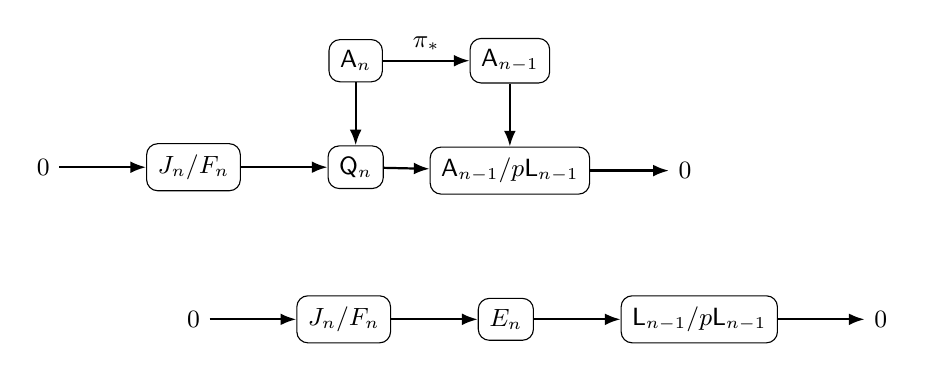
\begin{tikzpicture}[
  node distance=8mm and 11mm,
  every node/.style={font=\small},
  box/.style={draw,rounded corners,inner sep=4pt},
  arr/.style={-{Latex[length=2mm]},thick}
]
\node[box] (An) {$\A_n$};
\node[box,right=of An] (Ac) {$\A_{n-1}$};
\node[box,below=of An] (Qn) {$\QQ_n$};
\node[box,below=of Ac] (Cq) {$\A_{n-1}/p\LL_{n-1}$};
\draw[arr] (An)--node[above]{$\pi_*$}(Ac);
\draw[arr] (An)--(Qn);
\draw[arr] (Ac)--(Cq);
\draw[arr] (Qn)--(Cq);
\node[box,left=of Qn] (K) {$J_n/F_n$};
\node[left=of K] (zero1) {$0$};
\node[right=10mm of Cq] (zero2) {$0$};
\draw[arr] (zero1)--(K);
\draw[arr] (K)--(Qn);
\draw[arr] (Cq)--(zero2);
\node[below=14mm of K] (zero3) {$0$};
\node[box,right=of zero3] (K2) {$J_n/F_n$};
\node[box,right=of K2] (En) {$E_n$};
\node[box,right=of En] (sat) {$\LL_{n-1}/p\LL_{n-1}$};
\node[right=of sat] (zero4) {$0$};
\draw[arr] (zero3)--(K2);
\draw[arr] (K2)--(En);
\draw[arr] (En)--(sat);
\draw[arr] (sat)--(zero4);
\end{tikzpicture}
\caption{The canonical depth transition.  The upper square
records $\pi_*(\LL_n)=p\LL_{n-1}$ and the first quotient sequence; the lower
row isolates the additional saturation layer.}
\label{fig:depth-transition}
\end{figure}

\section{Depth two and the three residual invariants}\label{sec:S04}

At depth two abbreviate
\[
 \mathcal K_2=J_2/F_2,
 \qquad E_2=P_2/\LL_2.
\]
Let the point-fibre transfer be
\[
 \tau:\A_1\longrightarrow\A_2,\qquad
 \tau([a])=\sum_{\pi(x)=a}[x].
\]
Writing $\theta:E_2\to\LL_1/p\LL_1$ for the epimorphism in
\eqref{eq:second-depth-seq}, define
\begin{equation}\label{eq:mpupwp}
 m_p=\rank_{\F_p}(B_2),\qquad
 u_p=\dim_{\F_p}\theta(E_2[p]),\qquad
 w_p=\dim_{\F_p}(p^2\QQ_2).
\end{equation}

\begin{lemma}[Finite $p$-group profile recovery]
\label{lem:profile-recovery}
Let a full-rank inclusion of free abelian groups of rank $N$ have Smith
exponents $0,1,\ldots,h$ with multiplicities
$\nu_0,\nu_1,\ldots,\nu_h$.  If its finite cokernel is $G$, then
\begin{equation}\label{eq:profile-recovery}
 \sum_{i=0}^h\nu_i=N,\qquad
 \sum_{i=1}^h i\nu_i=\vp|G|,\qquad
 \nu_h=\dim_{\F_p}(p^{h-1}G).
\end{equation}
Consequently, an exponent-$p^2$ profile is fixed by $N$, $\nu_0$, and
$\vp|G|$; an exponent-$p^3$ profile is fixed by those data together with
$\dim_{\F_p}(p^2G)$.
\end{lemma}

\begin{proof}
In Smith coordinates,
$G\cong\bigoplus_{i=1}^h(\Z/p^i\Z)^{\nu_i}$.  Counting coordinates, taking
orders, and multiplying by $p^{h-1}$ give the three identities in
\eqref{eq:profile-recovery}.  For $h=2$ the first two are a nonsingular
two-equation system for $\nu_1,\nu_2$; for $h=3$ the last identity first fixes
$\nu_3$, leaving the same two-equation system.
\end{proof}

\begin{theorem}[Depth-two structural reduction]
\label{thm:depth-two-reduction}
For every prime $p$,
\[
 p^2P_2\subset\LL_2,\qquad p^3\A_2\subset\LL_2,
 \qquad \LL_2+p^2\A_2=\LL_2+\tau(\A_1).
\]
Consequently $E_2$, $\mathcal K_2$, and $\QQ_2$ have exponents at most $p^2$,
$p^2$, and $p^3$, respectively, and their complete profiles are determined
by $(m_p,u_p,w_p)$.  If unit factors are retained, the multiplicities for
$\LL_2\subset\A_2$ are
\begin{align}
 \mu_0&=m_p,\nonumber\\
 \mu_1&=p^4-2m_p+\frac{p(p^2+1)}2+w_p,\nonumber\\
 \mu_2&=m_p-\frac{p(p^2+1)}2-2w_p,\qquad \mu_3=w_p.
 \label{eq:q-from-mw}
\end{align}
For $E_2$ the nonunit multiplicities are
\begin{align}
 d_1&=\frac{p^2(2p^2+p+1)}2-2m_p,\nonumber\\
 d_2&=m_p-\frac{p^2(p+1)}2,\label{eq:E-from-m}
\end{align}
and for $\mathcal K_2$ they are
\begin{align}
 k_1&=\frac{p^2(2p^2+p+3)}2-2m_p-2u_p,\nonumber\\
 k_2&=m_p-\frac{p^2(p+3)}2+u_p.\label{eq:K-from-mu}
\end{align}
\end{theorem}

\begin{proof}
For a fine point $x$, let $S_x$ be the sum of all fine line rows through
$x$ and let $f_{\bar x}=\tau([\bar x])$.  Counting lines through pairs of
points gives the coefficientwise identity
\begin{equation}\label{eq:point-pencil}
 S_x=\mathbf1_{\A_2}+(p-1)f_{\bar x}+p^2[x].
\end{equation}
The all-one vector and every transferred coarse-line tube lie in $\LL_2$;
also $p\tau(\A_1)\subset\LL_2$ because $p\A_1\subset\LL_1$ at depth one.
Subtracting \eqref{eq:point-pencil} inside a point fibre gives
$p^2J_2\subset\LL_2$, because the point-basis differences inside the fibres
generate $J_2$.  For a coarse line $R$, choose one fine point above every
$\bar x\in R$ and write $\sigma(R)$ for their sum.  Summing
\eqref{eq:point-pencil} over these $p$ chosen points gives
\[
 \sum_{\bar x\in R}S_x
 =p\mathbf1_{\A_2}+(p-1)\tau(R)+p^2\sigma(R).
\]
The first two terms on the right lie in $\LL_2$, so
$p^2\sigma(R)\in\LL_2$.  Since the coarse line rows generate $\LL_1$, every
element of $P_2=\pi_*^{-1}(\LL_1)$ is a sum of an element of $J_2$ and such
section lifts.  This proves $p^2P_2\subset\LL_2$.

Equation \eqref{eq:point-pencil} also gives
$p^2\A_2\subset\LL_2+\tau(\A_1)$.  Conversely, for
$f\in\tau(\A_1)$ the same equation places $(p-1)f$ in
$\LL_2+p^2\A_2$, while $pf\in\LL_2$; hence
$f=pf-(p-1)f\in\LL_2+p^2\A_2$.  This proves the equality of superlattices.
Multiplying \eqref{eq:point-pencil} by $p$ and again using
$p\tau(\A_1)\subset\LL_2$ gives $p^3[x]\in\LL_2$ for every point $x$.

The equality
$\LL_2\cap p\A_2=\LL_2\cap pP_2$ follows by applying $\pi_*$ and cancelling
$p$ in the free lattice $\A_1$.  Hence the image ranks of $\LL_2$ in
$\A_2/p\A_2$ and in $P_2/pP_2$ coincide, so the unit Smith multiplicity for
both $\QQ_2=\A_2/\LL_2$ and $E_2=P_2/\LL_2$ is $m_p$.

We now apply \cref{lem:profile-recovery} rather than suppressing the profile
calculation.  From \eqref{eq:A-L-index} at $n=2$,
\[
 s_Q:=\vp|\QQ_2|=p^4-\frac{p(p^2+1)}2.
\]
Writing the four Smith multiplicities as $\mu_0,\ldots,\mu_3$, the preceding
paragraph and \eqref{eq:mpupwp} give
\[
 \mu_0=m_p,\qquad \mu_3=w_p,
 \qquad \mu_1+\mu_2=p^4-m_p-w_p,
 \qquad \mu_1+2\mu_2=s_Q-3w_p.
\]
Solving the last two equations gives exactly \eqref{eq:q-from-mw}.

The second exact sequence in \eqref{eq:second-depth-seq} specializes to
\begin{equation}\label{eq:depth-two-kernel-sequence}
 0\longrightarrow\mathcal K_2\longrightarrow E_2
 \xrightarrow{\theta}(\Z/p\Z)^{p^2}\longrightarrow0.
\end{equation}
The order formula in \cref{thm:canonical-depth-transition} gives
\[
 s_E:=\vp|E_2|=\frac{p^2(2p^2-p-1)}2.
\]
If $E_2\cong(\Z/p)^{d_1}\oplus(\Z/p^2)^{d_2}$, then
\[
 d_1+d_2=p^4-m_p,\qquad d_1+2d_2=s_E.
\]
Their unique solution is \eqref{eq:E-from-m}.

For completeness, put $v=p^2$ and
$u=\dim_{\F_p}\theta(E_2[p])=u_p$.  In bases adapted first to the restriction
of $\theta$ to the order-$p$ summands and then to its quotient image, $u$ of
the $d_1$ order-$p$ generators and $v-u$ of the $d_2$ order-$p^2$ generators
map to a basis of $(\Z/p)^v$.  The former leave $d_1-u$ order-$p$ kernel
generators; each of the latter leaves its $p$-multiple in the kernel; and the
unused order-$p^2$ generators remain unchanged.  Thus
\[
 \ker\theta\cong
 (\Z/p)^{d_1+v-2u}\oplus
 (\Z/p^2)^{d_2-v+u}.
\]
Substituting \eqref{eq:E-from-m}, $v=p^2$, and $u=u_p$ proves
\eqref{eq:K-from-mu} and completes the profile recovery.
\end{proof}

\section{Evaluation of the depth-two invariants}\label{sec:S05}

The modular rank is evaluated through the annihilator of the affine line
code.  The reduction needed for the complete-ideal calculation is recorded
explicitly first.

\begin{lemma}[Bundle-annihilator reduction]\label{lem:bundle-annihilator}
Put $k=\F_p$, $q=p^2$, and
\[
 A_k=k[(\Z/q\Z)^2]\cong k[x,y]/(x^q,y^q),
\]
where $x,y$ are augmentation coordinates.  Let $\mathcal I\subset A_k$ be
the modular affine-line code and let
$\mathcal J=\operatorname{Ann}_{A_k}(\mathcal I)$.  For each
$d\in\mathbb P^1(k)$ there is a regular parameter pair $(z_d,v_d)$, with
distinct tangent line $\ell_d=\operatorname{in}(z_d)=0$, such that
\begin{equation}\label{eq:bundle-annihilator}
 \mathcal J_d:=(z_d,v_d^p)^pA_k,
 \qquad \mathcal J=
 \bigcap_{d\in\mathbb P^1(k)}\mathcal J_d,
 \qquad m_p=\length_{A_k}(A_k/\mathcal J).
\end{equation}
\end{lemma}

\begin{proof}
If $H=\langle h\rangle$ is a primitive line subgroup, then in
characteristic $p$
\[
 N_H=\sum_{j=0}^{q-1}h^j=(h-1)^{q-1},
 \qquad \operatorname{Ann}_{A_k}(N_H)=(h-1)A_k.
\]
The translates of the $N_H$ generate $\mathcal I$.  The
coefficient-of-identity pairing makes $A_k$ a symmetric Frobenius algebra,
so annihilating the sum of the line ideals means annihilating every one:
\[
 \mathcal J=\bigcap_H(h-1)A_k,
 \qquad \dim_k\mathcal I=\dim_k(A_k/\mathcal J).
\]

Reduction modulo $p$ partitions the primitive directions into $p+1$
bundles, each containing $p$ lifts.  In the bundle over $d$, choose a group
basis $(g_d,t_d)$ for which the lifted line subgroups are generated by
\[
 h_{d,a}=g_dt_d^{pa}\quad(a\in k).
\]
Set $z_d=g_d-1$, $v_d=t_d-1$, and
$w_d=t_d^p-1=v_d^p$.  The subalgebra
\[
 C_d=k[z_d,w_d]/(z_d^q,w_d^p)
\]
has $A_k$ free over it with basis $1,v_d,\ldots,v_d^{p-1}$; hence finite
ideal intersections commute with extension from $C_d$ to $A_k$.  In $C_d$
write
\[
 f_{d,a}=(1+z_d)(1+w_d)^a-1=h_{d,a}-1.
\]
Modulo $(f_{d,a})$ one has
$z_d=(1+w_d)^{-a}-1$ and $w_d^p=0$, so every monomial of total
$(z_d,w_d)$-degree at least $p$ vanishes.  Thus
$(z_d,w_d)^p\subseteq\bigcap_a(f_{d,a})$.

For the reverse inclusion, pass to $C_d/(z_d,w_d)^p$.  The truncated
series
\[
 Z_d=\log(1+z_d),\qquad W_d=\log(1+w_d)
\]
use only the invertible denominators $1,\ldots,p-1$ and define a coordinate
automorphism.  Under it, $(f_{d,a})$ becomes the linear ideal
$(Z_d+aW_d)$.  A homogeneous polynomial of degree below $p$ lying in all
these $p$ distinct linear ideals is divisible by
$\prod_{a\in k}(Z_d+aW_d)$, of degree $p$, and is therefore zero.
Consequently
\[
 \bigcap_{a\in k}(h_{d,a}-1)A_k=(z_d,v_d^p)^pA_k.
\]
Intersecting these equalities over the $p+1$ coarse directions proves the
first part of \eqref{eq:bundle-annihilator}; the Frobenius dimension identity
proves the second.
\end{proof}

\begin{theorem}[Exact modular rank and thick-kernel profile]
\label{thm:modular-rank}
For every prime $p$,
\[
 m_p=\left(\frac{p(p+1)}2\right)^2.
\]
Consequently
\[
 E_2\cong
 (\Z/p\Z)^{p^3(p-1)/2}\oplus
 (\Z/p^2\Z)^{p^2(p^2-1)/4}.
\]
\end{theorem}

\begin{proof}
The exact modular object and its known upper-bound setting are those of
\L aba--Trainor and Dvir \cite{LT25,DVI26}; equality is established here by
the following complete-ideal calculation.  By
\cref{lem:bundle-annihilator}, it is enough to compute the colength of the
displayed annihilator.  Lift it to the complete regular local ring
$R=k[[x,y]]$, with maximal ideal $\mathfrak m=(x,y)$, and set
\[
 I_d=(z_d,v_d^p)^p,\qquad I=\bigcap_d I_d.
\]
A monomial outside $(z,v^p)^p$ satisfies
$a+\lfloor b/p\rfloor\leq p-1$, hence $a+b\leq p^2-1$.
Thus $\mathfrak m^{p^2}\subset I$, the Artinian truncation introduces no extra
ideal, and
\begin{equation}\label{eq:artinian-lift}
 \length_{A_k}(A_k/\mathcal J)=\length_R(R/I).
\end{equation}

The Newton inequality for $I_d$ is $pa+b\geq p^2$, so every $I_d$ is
integrally closed; their finite intersection $I$ is integrally closed as
well.  The complete-ideal/antinef result cited below is stated over an
algebraically closed residue field.  Let $\bar k$ be an algebraic closure of
$k$.  Because all the ideals contain $\mathfrak m^{p^2}$, scalar extension
may be performed in the finite-dimensional quotient $R/\mathfrak m^{p^2}$.
Faithful flatness makes it commute with the finite intersection, and
\[
 \dim_k(R/I)=
 \dim_{\bar k}\bigl(\bar k[[x,y]]/I\bar k[[x,y]]\bigr).
\]
We may therefore apply the geometric theorem after base change and descend
the resulting integer colength to $k$.

The resolution of each $(z,v^p)^p$ has multiplicity $p$ at the
origin and at a free chain of $p-1$ infinitely near points on the tangent
$z=0$.  The $p+1$ tangent lines are distinct, so the chains separate after
the first blow-up.  In the strict exceptional basis, the divisor of one
$I_d$ has coefficient $p$ at the root, coefficient $p(j+1)$ on its own
level-$j$ arm point, and coefficient $p$ on the other arms.  Intersecting
the global-section ideals takes the componentwise maximum.  Thus, on the
simultaneous star-shaped resolution, the divisor whose global-section ideal
is $I$ has root coefficient $p$ and coefficient $p(j+1)$ at level $j$ on
every arm.

The complete-ideal/antinef correspondence and the Hoskin--Deligne colength
formula are used in the precise form developed by Lipman and
Lipman--Watanabe \cite[Section~1]{LIP93}\cite[Corollary~1.1.2 and
Lemma~1.2]{LW03}.  For odd $p$, put
\[
 h=\frac{p-1}{2},\qquad A_0=\frac{p^2+2p-1}{2}.
\]
The least antinef majorant has strict exceptional coefficients
\[
 c_0=A_0,\qquad c_{d,j}=A_0+jh\quad(1\leq j\leq p-1),
\]
and therefore point basis $A_0$ at the root and $h$ at every arm point.
To see minimality, let $b_0,b_{d,j}$ be any antinef majorant and write
$u_{d,j}=b_{d,j}-b_{d,j-1}$.  Then
\[
 u_{d,1}\geq\cdots\geq u_{d,p-1}\geq0,\qquad
 b_0\geq\sum_d u_{d,1},\qquad b_{d,p-1}\geq p^2.
\]
If $b_0<A_0$, the endpoint bound forces every $u_{d,1}\geq h+1$, in
contradiction with the root inequality.  Discrete concavity along each arm
then places every $b_{d,j}$ above the chord $A_0+jh$.  This proves
minimality without a symmetry assumption.

When $p=2$, the unresolved divisor has strict coefficients $2$ at the root
and $4$ at each of the three endpoints.  If $b_0$ and $b_{d,1}$ are the
coefficients of an antinef majorant, then
$b_0\geq\sum_d(b_{d,1}-b_0)$, so $b_0\geq3$.  Root coefficient $3$ and
endpoint coefficients $4$ attain the bound; their point basis is $3$ at the
root and $1$ at each arm point.  Hoskin--Deligne now gives
\[
 \length(R/I)=
 \begin{cases}
 \binom42+3\binom22=9,&p=2,\\[2mm]
 \displaystyle
 \binom{A_0+1}{2}+(p+1)(p-1)\binom{h+1}{2}
 =\dfrac{p^2(p+1)^2}{4},&p\text{ odd}.
 \end{cases}
\]
Together with \eqref{eq:artinian-lift}, this proves the rank formula.
Substitution in \eqref{eq:E-from-m} proves the displayed profile.

We record why the same calculation also proves the initial-ideal equality
used later.  Put $S_0=k[X,Y]$ and, for the initial regular pair
$(\ell_d,m_d)$, set
\[
 I_d^{\mathrm{lin}}=(\ell_d,m_d^p)^p,\qquad
 I^{\mathrm{lin}}=\bigcap_d I_d^{\mathrm{lin}}.
\]
The ideals $I_d$ and $I_d^{\mathrm{lin}}$ have the same weighted proximity
graph: multiplicity $p$ at the origin followed by a free chain of $p-1$
points on tangent $d$.  Their intersections are complete ideals obtained by
the componentwise maximum of the branch divisors.  Although the actual and
linearized infinitely near points need not coincide, their common
star-shaped proximity graph and divisor coefficients are exactly the data
used by unloading and by Hoskin--Deligne.  The least antinef majorant computed
above therefore gives
\begin{equation}\label{eq:actual-linearized-colength}
 \length_R(R/I)=\length_{S_0}(S_0/I^{\mathrm{lin}})
 =\frac{p^2(p+1)^2}{4}.
\end{equation}

For the maximal-ideal filtration, finite colength gives
\[
 \length_R(R/I)=\length_{S_0}(S_0/\operatorname{in}I).
\]
On the other hand,
initial forms always give the inclusion
\[
 \operatorname{in}I\subseteq I^{\mathrm{lin}}
 =\bigcap_d\operatorname{in}I_d.
\]
The two quotients have equal finite length by
\eqref{eq:actual-linearized-colength}; hence the inclusion is equality.  Since
all ideals contain the relevant $p^2$-nd augmentation power, passage back to
the Artinian group-algebra quotient gives
\begin{equation}\label{eq:initial-intersection-equality}
 \operatorname{in}\!\left(\bigcap_d\mathcal J_d\right)
 =\bigcap_d\operatorname{in}(\mathcal J_d).
\end{equation}
Thus no general commutation rule for initial ideals and intersections is
being assumed.
\end{proof}

\begin{figure}[t]
\centering
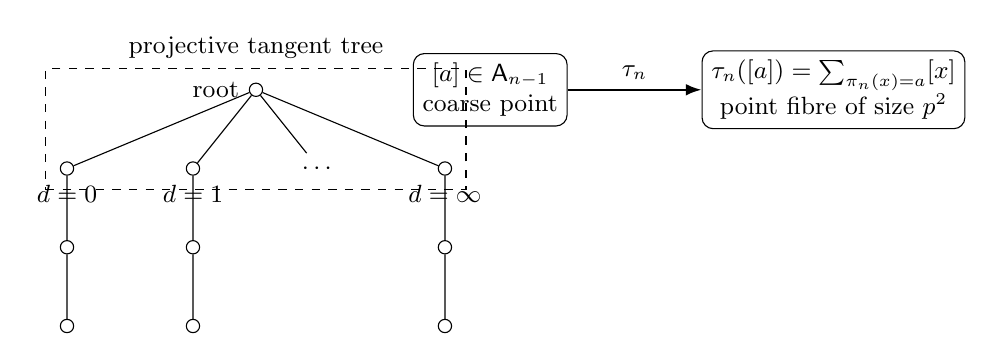
\begin{tikzpicture}[
  every node/.style={font=\small},
  level distance=10mm,
  sibling distance=16mm,
  arr/.style={-{Latex[length=2mm]},thick},
  dot/.style={circle,draw,inner sep=1.7pt}
]
\node[dot,label=left:{root}] (r) {}
 child {node[dot,label=below:{$d=0$}] (d0) {}
   child {node[dot]{} child {node[dot]{} }} }
 child {node[dot,label=below:{$d=1$}] (d1) {}
   child {node[dot]{} child {node[dot]{} }} }
 child {node[draw=none] (dots) {$\cdots$}}
 child {node[dot,label=below:{$d=\infty$}] (di) {}
   child {node[dot]{} child {node[dot]{} }} };
\node[draw,rounded corners,right=19mm of r,align=center] (coarse)
 {$[a]\in\A_{n-1}$\\coarse point};
\node[draw,rounded corners,right=17mm of coarse,align=center] (fibre)
 {$\tau_n([a])=\sum_{\pi_n(x)=a}[x]$\\point fibre of size $p^2$};
\draw[arr] (coarse)--node[above]{$\tau_n$}(fibre);
\node[draw,dashed,fit=(r)(d0)(d1)(di),inner sep=5pt,
 label=above:{projective tangent tree}] {};
\end{tikzpicture}
\caption{The $p+1$ separated tangent arms in the
complete-ideal calculation (left) and the point-fibre transfer used in the
reverse lattice intersection (right).  The two mechanisms evaluate $m_p$
and $w_p$, respectively.}
\label{fig:tangent-transfer}
\end{figure}

The remaining invariant $u_p$ controls only the fine kernel
$\mathcal K_2$, not the main quotient $\QQ_2$.  Its complete Bockstein and
filtered-interpolation proof is placed on the lateral branch in
\cref{app:saturation}; it is not an input to \cref{thm:depth-two-smith-profile}.

\begin{theorem}[Exact point-fibre transfer]
\label{thm:point-fibre-transfer}
For every prime $p$ and $n\geq2$,
\[
 \tau_n(\A_{n-1})\cap\LL_n=\tau_n(\LL_{n-1}).
\]
Consequently $\tau_n$ induces an injection
$\QQ_{n-1}\hookrightarrow\QQ_n$, and at depth two
\[
 w_p=\dim_{\F_p}(p^2\QQ_2)=\frac{p(p-1)}2.
\]
\end{theorem}

\begin{proof}
Let $\mathcal F_n:\A_n\to\OO_n$ be the maximal-order Fourier embedding and
write $\OO_n=\OO_{<n}\oplus\OO_{(n)}$.  A point fibre has $p^2$ points.
Character summation on its kernel gives
\begin{equation}\label{eq:transfer-fourier}
 \mathcal F_n(\tau_n(a))=
 p^2\iota_n(\mathcal F_{n-1}(a))\in\OO_{<n};
\end{equation}
the exact-order-$p^n$ component vanishes.  On the other hand,
\cref{thm:maximal-order-quotient} gives
\[
 \LL_n\cap\OO_{<n}
 =p^n(\mathsf M_n\cap\OO_{<n})
 =p^{n+1}\mathsf M_{n-1}.
\]
Since the ambient orders are torsion-free, cancellation in
\eqref{eq:transfer-fourier} yields
\[
 \tau_n(a)\in\LL_n
 \Longleftrightarrow
 \mathcal F_{n-1}(a)\in p^{n-1}\mathsf M_{n-1}
 \Longleftrightarrow a\in\LL_{n-1}.
\]
Distinct point fibres have disjoint support, so $\tau_n$ is injective.
At depth two, \cref{thm:depth-two-reduction} identifies $p^2\QQ_2$ with this transferred
copy of $\QQ_1$; the depth-one profile
$\QQ_1\cong(\Z/p\Z)^{p(p-1)/2}$ finishes the proof.
\end{proof}

\section{The all-prime depth-two Smith profile}\label{sec:S06}

\begin{theorem}[Depth-two Smith profile]
\label{thm:depth-two-smith-profile}
For every prime $p$, the inclusion $\LL_2\subset\A_2$ has unit
multiplicity
\[
 \mu_0=\frac{p^2(p+1)^2}{4},
\]
and
\begin{equation}\label{eq:main-profile}
 \QQ_2\cong
 (\Z/p\Z)^{p^3(p-1)/2}\oplus
 (\Z/p^2\Z)^{p(p-1)^2(p+2)/4}\oplus
 (\Z/p^3\Z)^{p(p-1)/2}.
\end{equation}
Equivalently, these are the nonunit Smith factors of $B_2$.
\end{theorem}

\begin{proof}
By \cref{thm:modular-rank,thm:point-fibre-transfer},
\[
 m_p=\frac{p^2(p+1)^2}{4},\qquad
 w_p=\frac{p(p-1)}2.
\]
Substitution of $m_p$ and $w_p$ into \eqref{eq:q-from-mw} gives the four
multiplicities in \cref{tab:smith-multiplicities}; deleting the unit factors gives
\eqref{eq:main-profile}.  Their weighted exponent sum equals
$p^4-p(p^2+1)/2$, independently matching \eqref{eq:A-L-index} at $n=2$.
\end{proof}

\begin{table}[t]
\centering
\caption{All-prime Smith multiplicities for
$\LL_2\subset\A_2$.}
\label{tab:smith-multiplicities}
\begin{tabular}{@{}lll@{}}
\toprule
Smith factor & multiplicity & role in $\QQ_2$\\
\midrule
$1$ & $p^2(p+1)^2/4$ & unit; omitted from the quotient\\
$p$ & $p^3(p-1)/2$ & exponent-one summands\\
$p^2$ & $p(p-1)^2(p+2)/4$ & exponent-two summands\\
$p^3$ & $p(p-1)/2$ & transferred depth-one carry\\
\bottomrule
\end{tabular}
\end{table}

\begin{table}[t]
\centering
\caption{Exact $p=2,3$ controls.  These rows are bounded computational
cross-checks, not the proof for all primes.}
\label{tab:finite-controls}
\begin{tabular}{@{}ccccc@{}}
\toprule
$p$ & unit & $p$-factor & $p^2$-factor & $p^3$-factor\\
\midrule
$2$ & $9$ & $4$ & $2$ & $1$\\
$3$ & $36$ & $27$ & $15$ & $3$\\
\bottomrule
\end{tabular}
\end{table}

The two rows of \cref{tab:finite-controls} are reconstructed by the exact local
validators described in \cref{sec:S09}.  They are deliberately presented
after the uniform proof and are not used to interpolate a law in $p$.

\section{Relative top shell, nonsplitting, and carry}\label{sec:S07}

Define the relative quotient and the exact top-shell projection by
\[
 \Rel_n=\QQ_n/\tau_n(\QQ_{n-1}),\qquad
 \lambda_n=\operatorname{pr}_{(n)}\mathcal F_n,\qquad
 \mathcal C_n=\lambda_n(\A_n)\subset\OO_{(n)}.
\]

\begin{theorem}[Relative top shell]
\label{thm:relative-top-shell}
For every prime $p$ and $n\geq2$,
\begin{gather}
 \ker\lambda_n=\tau_n(\A_{n-1}),\qquad
 \lambda_n(\LL_n)=p^n\OO_{(n)},\label{eq:top-kernel-image}\\
 \Rel_n\cong\mathcal C_n/p^n\OO_{(n)},\qquad
 p^n\Rel_n=0,\label{eq:relative-shell}
\end{gather}
and
\[
 \vp|\Rel_n|=
 \frac{p^{2n-2}\bigl(n(p^2-1)-p+1\bigr)}2.
\]
If a $\Z$-linear section of $\lambda_n$ is chosen, there is a homomorphism
\[
 \kappa_n:p^n\OO_{(n)}\longrightarrow\QQ_{n-1}
\]
such that
\begin{equation}\label{eq:kappa-graph}
 \QQ_n\cong
 (\QQ_{n-1}\oplus\mathcal C_n)
 \big/\langle(\kappa_n(c),c):c\in p^n\OO_{(n)}\rangle.
\end{equation}
Its class is independent of the section.
\end{theorem}

\begin{proof}
Equation \eqref{eq:transfer-fourier} gives the inclusion of the transfer
lattice in $\ker\lambda_n$.  Rationally both have dimension $p^{2n-2}$.
The transfer lattice is primitive in $\A_n$ because the all-one vector in
each point fibre extends to an integral basis; the kernel of a map to the
free lattice $\OO_{(n)}$ is also saturated.  Hence they agree.  The image
identity follows from
$\mathcal F_n(\LL_n)=p^n\mathsf M_n$ and the surjectivity
$\mathsf M_n\to\OO_{(n)}$.  This proves
\eqref{eq:top-kernel-image}--\eqref{eq:relative-shell}.

To derive rather than assume the top-shell normalization index, write the
index from \cref{lem:rational-decomposition} as
\[
 d_{p,m}:=\vp[\OO_m:\A_m]
 =\frac{mp^{2m}}2+
   \frac{(p+2)(p^{2m}-1)}{2(p^2-1)}.
\]
Inside $\OO_n=\OO_{<n}\oplus\OO_{(n)}$, the lower-tree intersection of
$\mathcal F_n(\A_n)$ is, by the kernel equality above and
\eqref{eq:transfer-fourier},
\[
 \mathcal F_n(\A_n)\cap\OO_{<n}
 =p^2\iota_n\bigl(\mathcal F_{n-1}(\A_{n-1})\bigr).
\]
The index of a full-rank lattice in a direct sum is the product of the index
of its projection and the index of its intersection with the kernel.
Consequently
\begin{align*}
 \vp[\OO_{(n)}:\mathcal C_n]
 &=d_{p,n}-d_{p,n-1}-2p^{2n-2}\\
 &=\frac{p^{2n-2}\bigl(n(p^2-1)+p-1\bigr)}2.
\end{align*}
Subtracting this from $n\rank\OO_{(n)}$, where
$\rank\OO_{(n)}=p^{2n}-p^{2n-2}$, gives the displayed order of $\Rel_n$.
Equivalently, the same exponent is
$\vp|\QQ_n|-\vp|\QQ_{n-1}|$ by
\cref{thm:maximal-order-quotient,thm:canonical-depth-transition}.
Finally, for $c\in p^n\OO_{(n)}$ choose $\ell\in\LL_n$ above $c$ and a
section lift $\sigma_n(c)$.  The unique $a$ satisfying
$\ell-\sigma_n(c)=\tau_n(a)$ defines $\kappa_n(c)=[a]$.  The transfer
intersection in \cref{thm:point-fibre-transfer} makes this well defined; the resulting
graph is exactly \eqref{eq:kappa-graph}.  A section change adds the usual
coboundary.
\end{proof}

\begin{corollary}[Nonsplitting]
\label{cor:nonsplitting}
For every prime $p$, the exact sequence
\[
 0\longrightarrow\QQ_1\longrightarrow\QQ_2
 \longrightarrow\Rel_2\longrightarrow0
\]
does not split.  In the exact finite cross-check $(p,n)=(2,3)$,
\begin{align*}
 \Rel_3&\cong(\Z/2)^{13}\oplus(\Z/4)^{12}\oplus(\Z/8)^9,\\
 E_3&\cong(\Z/2)^6\oplus(\Z/4)^{26}\oplus(\Z/8)^2,
\end{align*}
so equal order does not imply isomorphism.
\end{corollary}

\begin{proof}
At depth two, $\QQ_1$ has exponent $p$ and $\Rel_2$ has exponent at most
$p^2$, whereas \cref{thm:depth-two-smith-profile} gives $p(p-1)/2>0$ factors of order $p^3$
in $\QQ_2$.  A split extension cannot have such a factor.  For the second
statement, the exact top-shell and fibre-coordinate profiles are,
respectively,
\[
 0{:}9,1{:}12,2{:}13,3{:}14,
 \qquad 0{:}30,1{:}6,2{:}26,3{:}2.
\]
Reversing the top-shell profile as in \eqref{eq:relative-shell} and omitting
unit coordinates gives the displayed groups.  Both have order $2^{64}$,
but their images after multiplication by $4$ have dimensions $9$ and $2$.
This finite row is a counterexample to a universal identification, not an
all-depth formula.
\end{proof}

Put $q^\flat=p^{n-1}$ and $e=\varphi(q)=q-q^\flat$.  In the cyclic
polynomial order
$\mathscr R_q^X=\Z[X]/(X^q-1)$, let
\[
 \mathscr U_q^X=\langle1,X,\ldots,X^{e-1}\rangle_\Z,
 \qquad \mathfrak K_q^X=\Phi_q\mathscr R_q^X.
\]
The monic factorization $X^q-1=\Phi_q(X)(X^{q^\flat}-1)$ gives the unimodular
decomposition $\mathscr R_q^X=\mathscr U_q^X\oplus\mathfrak K_q^X$.
Since
$\tau_n(\A_{n-1})=\mathfrak K_q^X\otimes\mathfrak K_q^Y$, an integral
basis of the quotient is
\begin{equation}\label{eq:quotient-basis}
 \A_n/\tau_n(\A_{n-1})\cong
 (\mathscr U_q^X\otimes\mathscr R_q^Y)
 \oplus(\mathfrak K_q^X\otimes\mathscr U_q^Y).
\end{equation}

Here are the integral types of the two summands and their evaluation spaces.
Let $\mathcal O_q=\Z[\zeta_q]$ in the ordered power basis
$1,\zeta_q,\ldots,\zeta_q^{e-1}$, and put
\[
 D_1=\mathscr U_q^X\otimes\mathscr R_q^Y,
 \quad W_1=\mathcal O_q^{\oplus q},
 \qquad
 D_2=\mathfrak K_q^X\otimes\mathscr U_q^Y,
 \quad W_2=\mathcal O_q^{\oplus q^\flat}.
\]
All four are free abelian groups, with
\[
 \rank D_1=\rank W_1=eq,
 \qquad \rank D_2=\rank W_2=eq^\flat.
\]
The first-chart evaluation is an injective square $\Z$-linear map
$V_q^{(n)}:D_1\to W_1$; in $q\times q$ block notation its $(t,j)$ entry is
multiplication by $\zeta_q^{tj}$ on the common rank-$e$ power basis.  The
second diagonal evaluation is
$pV_{q^\flat}^{(n)}:D_2\to W_2$, with $(s,r)$ block multiplication by
$p\zeta_q^{psr}$.  Finally $X_{p,n}:D_1\to W_2$ is the cross-chart
evaluation.  Thus every block below denotes a homomorphism between specified
finite free $\Z$-modules, not an untyped scalar array.

\begin{theorem}[Two-chart block and clipped-line carry]
\label{thm:two-chart-block}
In integral bases compatible with \eqref{eq:quotient-basis}, the inclusion
$\mathcal C_n\subset\OO_{(n)}$ has the exact block presentation
\begin{equation}\label{eq:two-chart}
 T_{p,n}\sim
 \begin{pmatrix}
 V_q^{(n)}&0\\
 X_{p,n}&pV_{q^\flat}^{(n)}
 \end{pmatrix},
\end{equation}
where the displayed maps are expanded in the fixed integral bases just
specified.  The stable cross-chart datum is
\[
 \omega_{p,n}=[X_{p,n}]\in
 \operatorname{Ext}^1_{\Z}(\coker V_q^{(n)},
                            \coker(pV_{q^\flat}^{(n)})).
\]
There are compatible relation and carry matrices $\mathbf Z_{p,n}$ and
$\mathbf C^{\mathrm{car}}_{p,n}$ satisfying
\begin{equation}\label{eq:TZ}
 T_{p,n}\mathbf Z_{p,n}=\mathbf Z_{p,n}T_{p,n}=p^nI,
\end{equation}
with
\begin{equation}\label{eq:clipped-carry}
 (\mathbf C^{\mathrm{car}}_{p,n})_{(r,s);(u,j)}=
 \mathbf1_{\{u\cdot(e+r,e+s)=j\bmod q\}},
\end{equation}
where $(r,s)\in(\Z/q^\flat\Z)^2$, $u$ is a chart direction, and
$0\leq j<e$.  If
$U\mathbf Z_{p,n}V=\operatorname{diag}(p^{a_i})$, the extension is
represented by the columns $(\mathbf C^{\mathrm{car}}_{p,n}V)_i$ modulo
$p^{a_i}\QQ_{n-1}$.
\end{theorem}

\begin{proof}
For a basis monomial $X^iY^j$ in
$\mathscr U_q^X\otimes\mathscr R_q^Y$, evaluation at the two
direction charts gives
\[
 (1,t):\ \zeta_q^{i+tj},
 \qquad (ps,1):\ \zeta_q^{psi+j}.
\]
For $\Phi_q(X)X^rY^i$ in
$\mathfrak K_q^X\otimes\mathscr U_q^Y$, the corresponding values are
$0$ and $p\zeta_q^{psr+i}$, since
$\Phi_q(\zeta_q)=0$ and $\Phi_q(\zeta_q^{ps})=p$.  Stacking these rows
proves \eqref{eq:two-chart} by unimodular basis changes.

The exact elementary divisors of both diagonal cyclic blocks follow from
Weber--K\"unzer \cite[Proposition~3.15]{WK04}; Proposition~3.8 supplies a
diagonalization.  Explicitly, if $j=\sum a_kp^k$, their valuation
\[
 \beta_p(j)=\sum_{k\geq0}(a_k-a_{k+1})(k+1)p^k
\]
equals $\sum_{d=1}^jp^{v_p(d)}$ by digit telescoping.  Total ramification
multiplies the level-$(n-1)$ valuation by $p$, and the scalar $p$ adds
$\varphi(q)$.  This identifies the cited result with both diagonal blocks;
it does not remove $X_{p,n}$.

Set $A=V_q^{(n)}:D_1\to W_1$,
$B=pV_{q^\flat}^{(n)}:D_2\to W_2$, and $X=X_{p,n}:D_1\to W_2$.
Both $A$ and $B$ are injective: after tensoring with $\Q$ they are ordinary
Fourier evaluation isomorphisms, and their domains are torsion free.  Projection
to $W_1$ therefore induces the exact sequence of finite abelian groups
\begin{equation}\label{eq:two-chart-extension}
 0\longrightarrow\coker B
 \xrightarrow{\ [w_2]\mapsto[(0,w_2)]\ }
 \coker T_{p,n}
 \xrightarrow{\ [(w_1,w_2)]\mapsto[w_1]\ }
 \coker A\longrightarrow0.
\end{equation}
Indeed, if $[w_1]=0$, write $w_1=Ad_1$ and subtract
$T_{p,n}(d_1,0)$, leaving a class represented by $(0,w_2-Xd_1)$; injectivity
at the left follows because $Ad_1=0$ forces $d_1=0$.  This is also the exact
sequence obtained from the two length-one free resolutions by the snake
lemma.

A domain shear $D_1\to D_2$ and a codomain shear $W_1\to W_2$ replace the
cross map by
\[
 X\longmapsto X+BH+GA,\qquad
 H\in\operatorname{Hom}_{\Z}(D_1,D_2),\quad
 G\in\operatorname{Hom}_{\Z}(W_1,W_2).
\]
Conversely, these are precisely the changes of representative obtained from
such integral splittings.  Since $A$ and $B$ are injective presentations by
finite free $\Z$-modules, the standard presentation quotient is
\[
 \frac{\operatorname{Hom}_{\Z}(D_1,W_2)}
 {B\operatorname{Hom}_{\Z}(D_1,D_2)
  +\operatorname{Hom}_{\Z}(W_1,W_2)A}
 \cong
 \operatorname{Ext}^1_{\Z}(\coker A,\coker B).
\]
Thus $[X_{p,n}]$ is exactly the extension class of
\eqref{eq:two-chart-extension}, with its category and integral bases fixed.

Finally extend \eqref{eq:quotient-basis} by
$\mathfrak K_q^X\otimes\mathfrak K_q^Y$ to a unimodular basis of $\A_n$.
Choose, for each $(u,j)$, the affine-line indicator
$W_{u,j}$ with $0\leq j<e$.  To make the coordinate passage explicit, write
$L_{u,j}(x,y)=\mathbf1_{\{u\cdot(x,y)=j\bmod q\}}$ and
$\widehat t=e+(t\bmod q^\flat)$.  Pointwise on $(\Z/q\Z)^2$ one has the
telescoping identity
\[
\begin{split}
L_{u,j}(x,y)={}&\mathbf1_{\{x<e\}}
  \bigl(L_{u,j}(x,y)-L_{u,j}(\widehat x,y)\bigr)\\
&+\mathbf1_{\{y<e\}}
  \bigl(L_{u,j}(\widehat x,y)-L_{u,j}(\widehat x,\widehat y)\bigr)
  +L_{u,j}(\widehat x,\widehat y).
\end{split}
\]
The first two terms are precisely the $D_1$- and $D_2$-coordinates of
$\mathbf Z_{p,n}$, while the last term is the high--high coordinate
\eqref{eq:clipped-carry}.  The top Fourier image of $W_{u,j}$ is
$q\zeta_q^j$ in the $u$-component and zero elsewhere, so stacking these
coordinate columns gives $T_{p,n}\mathbf Z_{p,n}=qI$.  Both matrices are
square; over $\Q$ this says $\mathbf Z_{p,n}=qT_{p,n}^{-1}$ and therefore
$\mathbf Z_{p,n}T_{p,n}=qI$ as an integral equality, proving
\eqref{eq:TZ}.  A Smith change of relation basis sends
$\mathbf C^{\mathrm{car}}_{p,n}$ to $\mathbf C^{\mathrm{car}}_{p,n}V$, and
the relation $p^{a_i}$ makes its $i$th column well defined modulo
$p^{a_i}\QQ_{n-1}$.
\end{proof}

\begin{corollary}[Depth-two first filtered rank]
\label{cor:depth-two-filtered-rank}
For the two-chart class at depth two,
\[
 d_0(2,2)=0,
 \qquad d_0(p,2)=\frac{(p-1)^2(p+1)}8\quad(p\text{ odd}).
\]
\end{corollary}

\begin{proof}
The first filtered rank of the cross-chart class in
\cref{thm:two-chart-block} is
\[
 d_0(p,n)=\rank_{\F_p}
 \begin{pmatrix}\overline{V_q^{(n)}}\\\overline{X_{p,n}}\end{pmatrix}
 -\rank_{\F_p}\overline{V_q^{(n)}}.
\]
At $n=2$, the diagonal unit count is determined by the two
Weber--K\"unzer blocks in \cref{thm:two-chart-block}; subtracting it from the total
unit multiplicity $\mu_0$ in \cref{thm:depth-two-smith-profile} gives the displayed values.
Thus the corollary, unlike the two-chart construction itself, depends on the
depth-two Smith theorem.
\end{proof}

\begin{figure}[t]
\centering
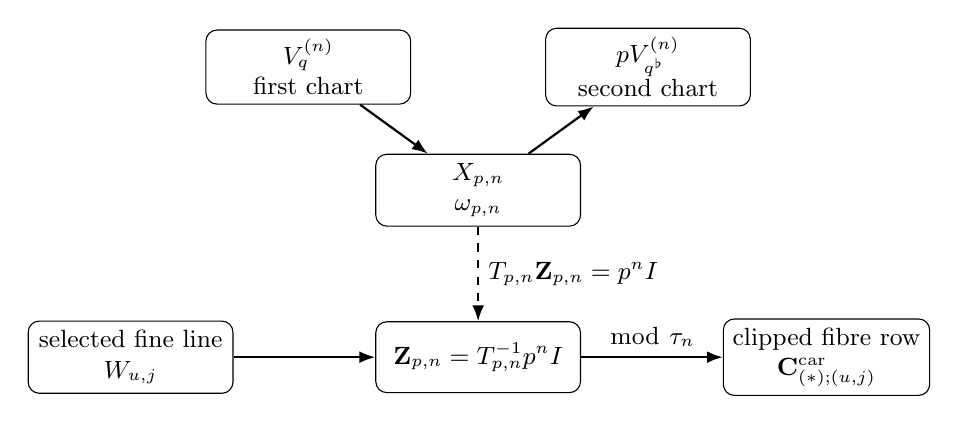
\begin{tikzpicture}[
  every node/.style={font=\small},
  box/.style={draw,rounded corners,minimum width=26mm,minimum height=9mm,
              align=center},
  arr/.style={-{Latex[length=2mm]},thick}
]
\node[box] (V) {$V_q^{(n)}$\\first chart};
\node[box,right=17mm of V] (pV) {$pV_{q^\flat}^{(n)}$\\second chart};
\node[box,below=11mm of $(V)!0.5!(pV)$] (X)
 {$X_{p,n}$\\$\omega_{p,n}$};
\draw[arr] (V)--(X);
\draw[arr] (X)--(pV);
\node[box,below=12mm of X] (Z)
 {$\mathbf Z_{p,n}=T_{p,n}^{-1}p^nI$};
\node[box,left=18mm of Z] (line) {selected fine line\\$W_{u,j}$};
\node[box,right=18mm of Z] (Ccar)
 {clipped fibre row\\$\mathbf C^{\mathrm{car}}_{(*);(u,j)}$};
\draw[arr] (line)--(Z);
\draw[arr] (Z)--node[above]{$\bmod\ \tau_n$}(Ccar);
\draw[arr,dashed] (X)--node[right]{$T_{p,n}\mathbf Z_{p,n}=p^nI$}(Z);
\end{tikzpicture}
\caption{The two cyclic charts are glued by
$\omega_{p,n}$; in the same integral basis the relation inverse transports a
selected fine line to the clipped-line carry.}
\label{fig:two-chart-carry}
\end{figure}

\section{Filtered all-depth perspective and its limits}\label{sec:S08}

The two-chart class admits a standard filtered description.  Work over
$\Z_p$ and let $A:D_A\to V_A$ and $B:D_B\to V_B$ be injective square
lattice maps.  For $r\geq0$, put
\[
 M_r(A)=\{x\in D_A:Ax\in p^rV_A\},
 \qquad \Lambda_r(A)=\log_p[D_A:M_r(A)].
\]
For
\(
 H=\begin{psmallmatrix}A&0\\X&B\end{psmallmatrix}
\)
define
\[
 \Omega_r:M_r(A)\longrightarrow V_B/(BD_B+p^rV_B),
 \qquad x\longmapsto[Xx],
\]
and $\eps_r(H)=\log_p|\im\Omega_r|$, with $\eps_0=0$.

\begin{proposition}[Filtered obstruction identity and companion boundary]
\label{prop:filtered-obstruction}
For every $r\geq1$,
\begin{equation}\label{eq:filtered-index}
 \Lambda_r(H)=\Lambda_r(A)+\Lambda_r(B)+\eps_r(H).
\end{equation}
If the Smith exponents of an injective map $F$ lie in $[0,R]$, their
multiplicities are recovered from
\begin{align*}
 m_0(F)&=\Lambda_1(F),\\
 m_h(F)&=\Lambda_{h+1}(F)-2\Lambda_h(F)+\Lambda_{h-1}(F)
       &&(1\leq h<R),\\
 m_R(F)&=\rank(F)-\Lambda_R(F)+\Lambda_{R-1}(F).
\end{align*}
Applied to \eqref{eq:two-chart}, the finite list
$\eps_r(T_{p,n})$, $1\leq r\leq n$, determines the top-shell profile.
Together with the carry block, the same identity yields an exact full-size
recursive presentation.  This last construction is a methods/software
companion: it is not an independent geometry constructor, a reduced-rank
algorithm, or a headline theorem of this manuscript.
\end{proposition}

\begin{proof}
A pair $(x,y)$ lies in $M_r(H)$ exactly when
\[
 Ax\in p^rV_A,\qquad Xx+By\in p^rV_B.
\]
The first condition places $x$ in $M_r(A)$; the second has a solution if and
only if $x\in\ker\Omega_r$, and two solutions differ by $M_r(B)$.  Hence
\[
 0\longrightarrow M_r(B)\longrightarrow M_r(H)
 \longrightarrow\ker\Omega_r\longrightarrow0.
\]
Taking indices proves \eqref{eq:filtered-index}.  In Smith coordinates,
$\Lambda_r(F)=\sum_i\max(r-a_i,0)$, and the displayed finite differences
recover the multiplicities.

The filtration and multiplicity-recovery layer is stated directly by Sin
\cite[Section~2.1, equations~(4)--(8)]{SIN14}.  Moreover, $\Omega_r$ is the
coordinate form of the ordinary connecting morphism
\[
 \coker(A)[p^r]\longrightarrow\coker(B)/p^r\coker(B)
\]
in the long exact Tor sequence \cite[Lemma~10.75.2]{STK-TOR}.  Thus the
abstract mechanism receives no originality credit here.  The domain-specific
companion computes its image lattices on the fixed affine incidence geometry and transports
integral bases through
\[
 \mathcal B_n=
 \begin{pmatrix}\mathcal B_{n-1}&\Xi_n\\0&\mathbf Z_{p,n}\end{pmatrix},
\]
where $\mathcal B_n$ is the typed basis-transport matrix and $\Xi_n$ its
carry-coupling block; neither symbol denotes the preimage lattice $P_n$ or
the cyclotomic ideal $\mathfrak K_q^X$.
That realization runs at ambient rank $p^{2n}$ and relies on the separately
fixed two-chart geometry.  Broad recursion through Hjelmslev levels is also
known geometrically \mbox{\cite{HVM89,KOH09}}.  No reduction of asymptotic work and
no uniform explicit all-depth profile is asserted.
\end{proof}

\section{Sources, limitations, and computational role}\label{sec:S09}

The proof of the exact affine integer statement is given in
\cref{thm:depth-two-smith-profile}.  The sources in \cref{tab:source-boundary} delimit the imported
object, cyclic, local-algebra, and extension layers; ``proved here'' never
means a literature-wide firstness claim.

\begin{table}[t]
\centering
\small
\caption{Compact source and nontransfer boundary.}
\label{tab:source-boundary}
\begin{tabular}{@{}>{\raggedright\arraybackslash}p{0.24\textwidth}
                    >{\raggedright\arraybackslash}p{0.26\textwidth}
                    >{\raggedright\arraybackslash}p{0.39\textwidth}@{}}
\toprule
Layer & Sources & Boundary used here\\
\midrule
Affine transform and depth one & \cite{MOL12,ILM,CSX06} & context and
field-depth factors; no new ownership\\
Maximal-order branch CRT & \cite{MS15} & cyclic layer imported; tree
assembly proved in \cref{thm:maximal-order-quotient}\\
Modular rank and complete ideals & \cite{LT25,DVI26,LIP93,LW03} & exact
object/bounds and local-algebra machinery attributed; application proved in
\cref{thm:modular-rank}\\
Level geometry & \cite{LV14,KOH09,HVM89} & broad projective rank and lift
geometry only; no integral affine transfer\\
Cyclic diagonal blocks & \cite{WK04} & both diagonal Smith formulas are
prior art; the cross-chart class and carry remain\\
Filtered extension layer & \cite{SIN14,STK-TOR} & standard-derived identity;
domain-specific realization is supporting only\\
Unavailable exact text & \cite{LAN17,BLR23} & metadata/abstract scope only;
no theorem or matrix passage is imported\\
\bottomrule
\end{tabular}
\end{table}

The source search was bounded and is not a completeness certificate.  Exact
text and conventions for \cite{LAN17,BLR23} were unavailable; no projective
matrix is identified with $B_2$, no modular rank is promoted to an integer
Smith profile, and no originality or priority conclusion is drawn.  The
software reproduces closed exact controls, rejects typed and lattice
mutations, and evaluates the full-size companion construction.  It is
bounded computational cross-checking, not a substitute for any all-parameter proof; no $(5,2)$ result or
unexecuted generic-orbit experiment enters this manuscript.

\section{Reproducibility and companion interface}\label{sec:S10}

The theorem proofs are contained in the manuscript.  The repository companion
has the narrower roles in \cref{tab:companion-interface}.  It is self-contained, uses exact
integer arithmetic through SymPy, makes no network requests, and writes no
scientific result files.

\begin{table}[t]
\centering
\small
\caption{Compact companion interface.}
\label{tab:companion-interface}
\begin{tabular}{@{}>{\raggedright\arraybackslash}p{0.19\textwidth}
                    >{\raggedright\arraybackslash}p{0.31\textwidth}
                    >{\raggedright\arraybackslash}p{0.39\textwidth}@{}}
\toprule
Layer & Reproduced object & Evidentiary boundary\\
\midrule
Exact controls & closed Smith profiles and index identities & bounded
arithmetic cross-checks only; no finite extrapolation\\
Hostile tests & prime types, lattice equalities, and fail-closed boundaries &
rejects invalid primes, strict-sublattice mutations, and the reserved target\\
Full-size companion & filtered image lattices and carry transport & exact
supporting realization on fixed geometries; no finite extrapolation or
compression claim\\
Build checks & source manifest, release digest, and clean PDF & integrity and
visual evidence, not mathematical proof\\
\bottomrule
\end{tabular}
\end{table}

From the repository root, the exact arithmetic receipt is printed by
\begin{verbatim}
python -B companion/affine_hjelmslev_radon_smith.py
\end{verbatim}
and the hostile and differential controls are run by
\begin{verbatim}
 python -B -m pytest -q -p no:cacheprovider \
   --basetemp /tmp/fcig-hjelmslev-pytest tests
\end{verbatim}
The two package-integrity layers are checked with
\begin{verbatim}
python -B scripts/check_manifest.py
python -B scripts/check_release.py
\end{verbatim}
The paper is built from \path{paper/main.tex} with LuaLaTeX, Biber, and
\texttt{latexmk}; \path{REPRODUCE.md} records the fixed-epoch command and
the precise environment boundary.  The repository ships the title-named PDF.
Its build and the finite computations provide reproducibility evidence only.
The PDF catalog declares English and the public source preserves semantic
section, theorem, equation and table structure.  PDF/UA conformance is not
claimed; the exact accessibility boundary is recorded in
\path{ACCESSIBILITY.md}.

\appendix

\section{Saturation and augmentation: the lateral fine-kernel branch}
\label{app:saturation}

Let $C_i$ be the free abelian group on depth-$i$ affine lines and let
$\partial_i:C_i\to\A_i$ be incidence.  Reduction of lines gives
$\gamma:C_2\to C_1$ and
\begin{equation}\label{eq:bockstein-square}
 \pi_*\partial_2=p\partial_1\gamma.
\end{equation}

\begin{lemma}[Bockstein image and dual criterion]
\label{lem:bockstein-dual}
The image $H_p:=\theta(E_2[p])\subset\LL_1/p\LL_1$ is exactly the image of
\begin{equation}\label{eq:bockstein-map}
 \ker(\partial_2\bmod p)\longrightarrow\LL_1/p\LL_1,
 \qquad c\longmapsto\partial_1\gamma(c)\bmod p\LL_1.
\end{equation}
If $Y=(\LL_1/p\LL_1)^*$, $\rho$ reduces fine lines, and
$\mathsf{Col}_2=\im(\partial_2^{\transpose}\bmod p)$ is the
fine column code, then
\begin{equation}\label{eq:dual-criterion}
 y\text{ annihilates }H_p
 \quad\Longleftrightarrow\quad \rho^*y\in\mathsf{Col}_2.
\end{equation}
\end{lemma}

\begin{proof}
If $c\bmod p\in\ker(\partial_2\bmod p)$, write
$\partial_2c=px$.  Cancellation in the free lattice in
\eqref{eq:bockstein-square} gives
$\pi_*x=\partial_1\gamma(c)$.  Conversely, every class in $E_2[p]$ has a
representative $x$ with $px\in\LL_2$, so choosing $c$ with
$\partial_2c=px$ recovers it in this way.  This proves
\eqref{eq:bockstein-map}.

A line-coordinate vector represents an element of $Y$ precisely when its
sum on a parallel class is independent of the direction.  Indeed, the
differences of the $p+1$ complete parallel-class sums give $p$ integral
relations, and the coarse point Gram matrix $pI+J$ is nonsingular over
$\Q$, so these have the full relation rank.  Pairing
\eqref{eq:bockstein-map} with $y$ gives
\[
 \langle y,\partial_1\gamma(c)\rangle
 =\langle\rho^*y,c\rangle.
\]
Finite-dimensional orthogonality
$(\ker\partial_2)^\perp=\im\partial_2^{\transpose}$ proves
\eqref{eq:dual-criterion}.
\end{proof}

\begin{lemma}[Uniform fibre span]\label{lem:fibre-span}
The subspace $H_p$ has dimension at most one.
\end{lemma}

\begin{proof}
For a coarse point $a$, let $P_a$ be its line-coordinate pencil.  For a
coarse direction $d$, let $R_d(a)$ be the line of direction $d$ through
$a$.  Identify the point fibre over $a$ with $k^2$, choose a nonzero
functional $\beta$ with kernel $d$, and give the fibre point $b$ weight
$-\beta(b)^{p-1}$.  A fine line in direction $d$ has weight sum zero;
otherwise $\beta$ runs through $k$ and
$-\sum_{t\in k}t^{p-1}=1$.  Its fine Radon transform is therefore
\[
 \rho^*(P_a-e_{R_d(a)})\in\mathsf{Col}_2.
\]

These vectors span the total-coordinate-sum-zero hyperplane $W_0$.  To see
this, a vector orthogonal to all of them has equal values on all lines
through each point.  Intersecting nonparallel lines, and connecting parallel
lines by a transversal, forces the vector to be constant; conversely
constants are orthogonal to every displayed generator.  Thus
$Y\cap W_0\subset H_p^\perp$ by \eqref{eq:dual-criterion}.  For $y\in Y$,
the common parallel sum equals the total coordinate sum because
$p+1=1$ in $k$, while $P_a$ has common sum one.  Hence $Y\cap W_0$ has
codimension one in $Y$, proving the lemma.
\end{proof}

\begin{theorem}[Saturation and augmentation]
\label{thm:saturation-augmentation}
The saturation invariant is
\[
 u_p=0\quad\text{for odd }p,\qquad u_2=1.
\]
Thus
\[
 \mathcal K_2\cong
 \begin{cases}
 (\Z/p\Z)^{p^2(p^2-p+2)/2}\oplus
 (\Z/p^2\Z)^{p^2(p^2-5)/4},&p\text{ odd},\\
 (\Z/2\Z)^6,&p=2.
 \end{cases}
\]
\end{theorem}

\begin{proof}
By \cref{lem:fibre-span}, it remains to decide one point pencil.  In the
bundle coordinates of \cref{lem:bundle-annihilator}, the kernel of the fine
Radon map on bundle $d$ is $\mathcal J_d$.  The diagonal quotient map
$A_k\to\bigoplus_d A_k/\mathcal J_d$ therefore shows that
$\rho^*P_0\in\mathsf{Col}_2$ is equivalent to the existence of an
$f\in A_k$ satisfying the simultaneous congruences
\begin{equation}\label{eq:pencil-congruences}
 f\equiv v_d^D\pmod{(z_d,v_d^p)^p}
 \quad(d\in\mathbb P^1(k)),\qquad D=p(p-1).
\end{equation}
Indeed, in a direction bundle the fine offsets reducing through the origin
form the order-$p$ subgroup, whose norm is
\[
 \sum_{j=0}^{p-1}t_d^{pj}=(t_d^p-1)^{p-1}=v_d^D.
\]

Filter $A_k$ by augmentation degree.  Its associated graded ring is
\[
 S=k[X,Y]/(X^{p^2},Y^{p^2}).
\]
For a regular linear pair $(\ell_d,m_d)$,
\[
 \operatorname{in}(z_d,v_d^p)^p=(\ell_d,m_d^p)^p.
\]
A monomial $\ell_d^am_d^b$ survives precisely when
$a+\lfloor b/p\rfloor\leq p-1$.  Consequently, in degree $D$ the surviving
classes are $m_d^D$ and $\ell_dm_d^{D-1}$; in every degree
$D<e\leq p^2-1$ only $m_d^e$ survives, and there is no quotient component
above degree $p^2-1$.

Assume first that $p$ is odd.  With
$\ell_a=Y-aX,m_a=X$ for $a\in k$ and
$\ell_\infty=X,m_\infty=Y$, use the degree-$D$ form
\[
 F_D(X,Y)=X^D+Y^D-2X^{p-1}Y^{D-p+1}
              +X^{2p-2}Y^{D-2p+2}.
\]
On $X=1$,
\[
 F_D(1,T)=1+T^{D-2p}(T^p-T)^2.
\]
Thus its value is one and its first derivative is zero at every finite
$k$-point; the coefficients of $Y^D$ and $XY^{D-1}$ give the same value and
first-jet conditions at infinity.  It solves the initial degree of every
congruence in \eqref{eq:pencil-congruences}.

After subtracting a lift of $F_D$, suppose the first residual degree is
$e>D$.  Each local quotient is then one-dimensional, so its symbol is an
arbitrary list of $p+1$ values on $\mathbb P^1(k)$.  Evaluation of degree-$e$
binary forms is onto: for each point $d$, take the product of the $p$ linear
forms vanishing at all other rational points, normalize its nonzero value at
$d$, and multiply by a degree-$(e-p)$ form nonvanishing at $d$.  These are a
Lagrange basis.  Lift the resulting form and subtract again.  Each step
strictly raises the residual degree, and the local quotients vanish above
$p^2-1$; the process therefore terminates after finitely many steps and
solves all actual, not merely initial, congruences.  Hence
$\rho^*P_0\in\mathsf{Col}_2$ and
\eqref{eq:dual-criterion} gives $H_p=0$ for odd $p$.

For $p=2$, we spell out the strictness consequence of
\eqref{eq:initial-intersection-equality}.  Give
\[
 \Phi:A_k\longrightarrow\bigoplus_d A_k/\mathcal J_d,
 \qquad f\longmapsto(f\bmod\mathcal J_d)_d
\]
the augmentation filtrations.  Then
\[
 \ker(\operatorname{gr}\Phi)=\bigcap_d\operatorname{in}(\mathcal J_d),
 \qquad
 \operatorname{gr}(\ker\Phi)
 =\operatorname{in}\!\left(\bigcap_d\mathcal J_d\right),
\]
so \eqref{eq:initial-intersection-equality} identifies these two spaces.
If $\Phi(f)$ has filtration degree at least $r$ but $f$ has initial degree
$s<r$, its degree-$s$ symbol lies in $\ker(\operatorname{gr}\Phi)$ and is
therefore the initial symbol of some $h\in\ker\Phi$.  Replacing $f$ by $f-h$
preserves its image and raises its initial degree.  Iteration terminates in
the finite augmentation filtration and produces a preimage in degree at
least $r$.  Hence $\Phi$ is strict.

The right side of \eqref{eq:pencil-congruences} starts in degree $D=2$.
Strictness shows that any hypothetical preimage may be chosen with quadratic
initial form $aX^2+bXY+cY^2$.  The value and first-jet conditions at $0$ and
$\infty$ require $a=c=1$ and $b=0$.  At the third tangent
$\ell=Y-X,m=X$, the same conditions require $a+b+c=1$ and $b=0$, contradicting
$a+b+c=0$ in $\F_2$.  Thus the pencil is not in the fine column code.  Hence
$H_2\ne0$, while \cref{lem:fibre-span} gives $\dim H_2\leq1$.  Moreover, the
total-coordinate-sum-zero subspace $Y\cap W_0$ is exactly the annihilator of
the all-one class in $\LL_1/2\LL_1$.  Therefore $H_2$ is exactly that
augmentation line.
Therefore $u_2=1$.  Substitution in \eqref{eq:K-from-mu} gives the stated
profiles of $\mathcal K_2$.
\end{proof}

\printbibliography

\end{document}
